
\begin{figure}[H]
    \renewcommand{\figurename}{Рисунок}
    \centering{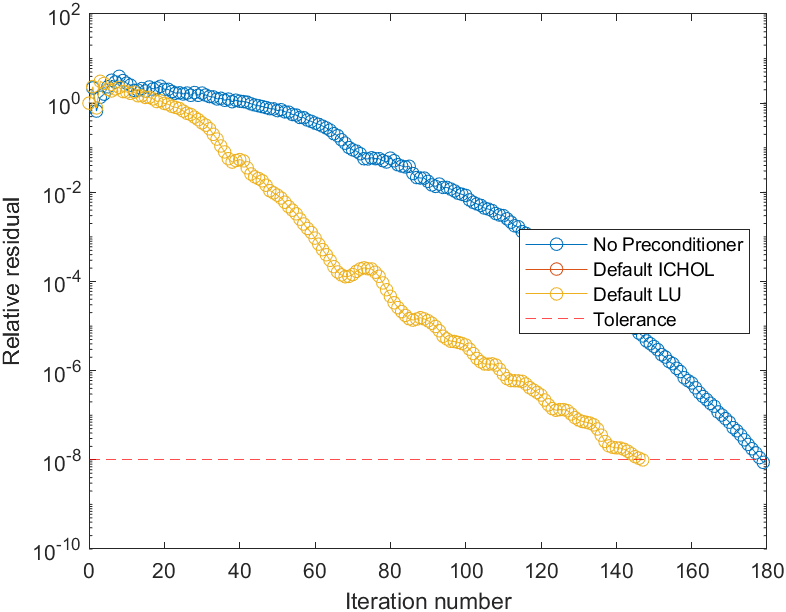
\includegraphics[scale=0.70]{img/dupcova/bicg}}
    \caption{История невязок методом bicg для матрицы Dubcova2}
    \label{fig:image_1}
\end{figure}

\begin{figure}[H]
    \renewcommand{\figurename}{Рисунок}
    \centering{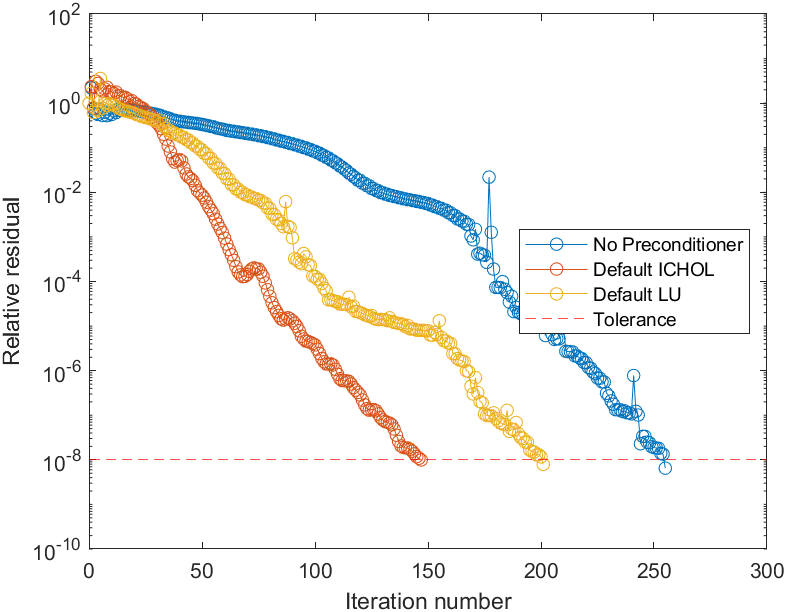
\includegraphics[scale=0.70]{img/dupcova/bicgstab}}
    \caption{История невязок методом bicgstab для матрицы Dubcova2}
    \label{fig:image_2}
\end{figure}

\begin{figure}[H]
    \renewcommand{\figurename}{Рисунок}
    \centering{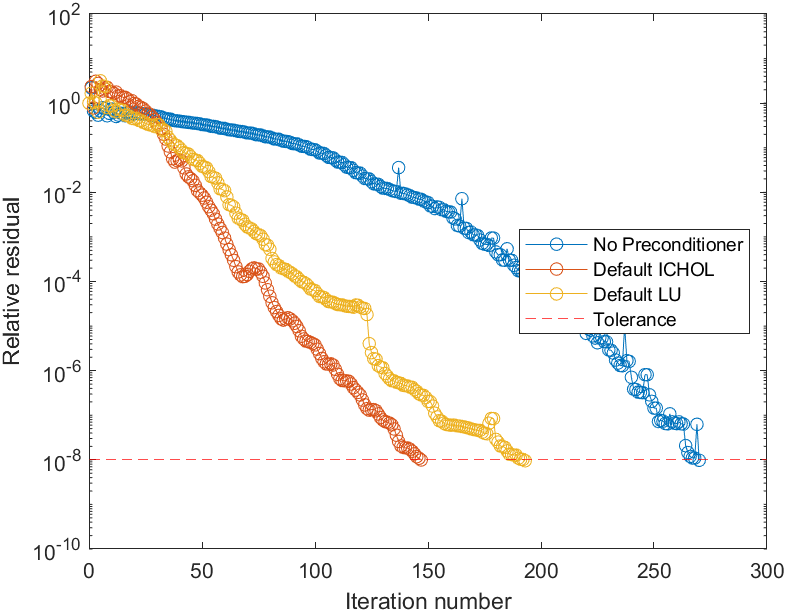
\includegraphics[scale=0.70]{img/dupcova/bicgstabl}}
    \caption{История невязок методом bicgstabl для матрицы Dubcova2}
    \label{fig:image_3}
\end{figure}

\begin{figure}[H]
    \renewcommand{\figurename}{Рисунок}
    \centering{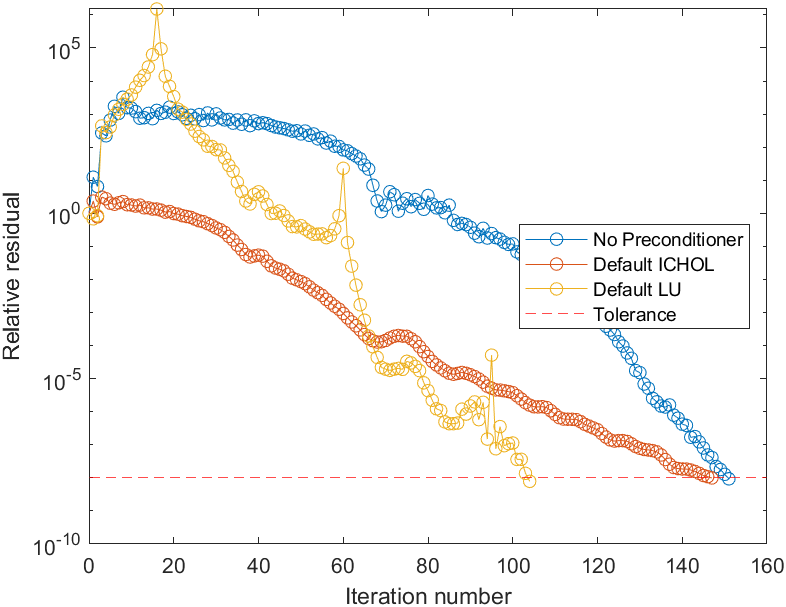
\includegraphics[scale=0.70]{img/dupcova/cgs}}
    \caption{История невязок методом cgs для матрицы Dubcova2}
    \label{fig:image_4}
\end{figure}

\begin{figure}[H]
    \renewcommand{\figurename}{Рисунок}
    \centering{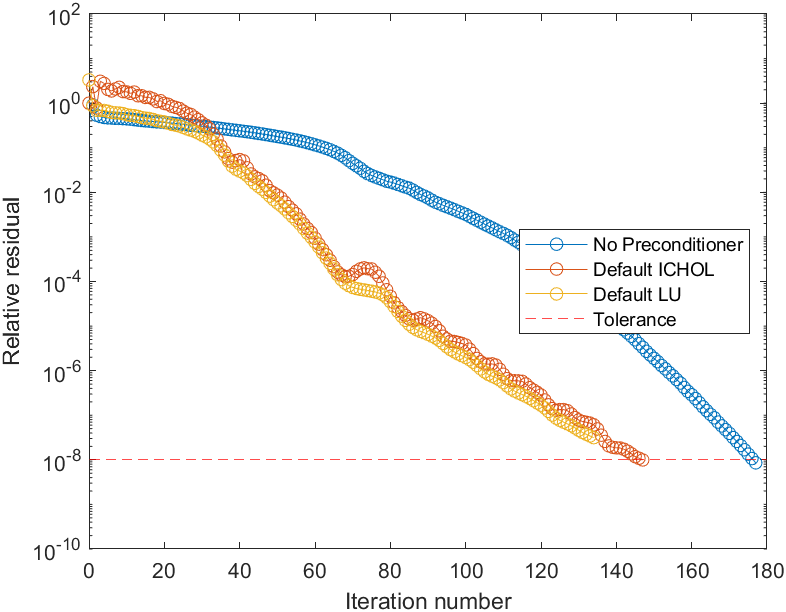
\includegraphics[scale=0.70]{img/dupcova/gmres}}
    \caption{История невязок методом gmres для матрицы Dubcova2}
    \label{fig:image_5}
\end{figure}

\begin{figure}[H]
    \renewcommand{\figurename}{Рисунок}
    \centering{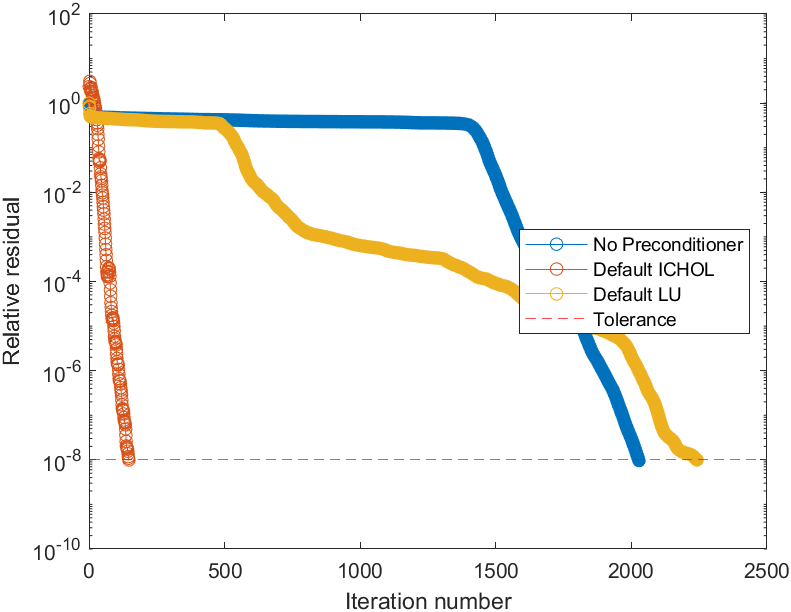
\includegraphics[scale=0.70]{img/dupcova/lsqr}}
    \caption{История невязок методом lsqr для матрицы Dubcova2}
    \label{fig:image_6}
\end{figure}

\begin{figure}[H]
    \renewcommand{\figurename}{Рисунок}
    \centering{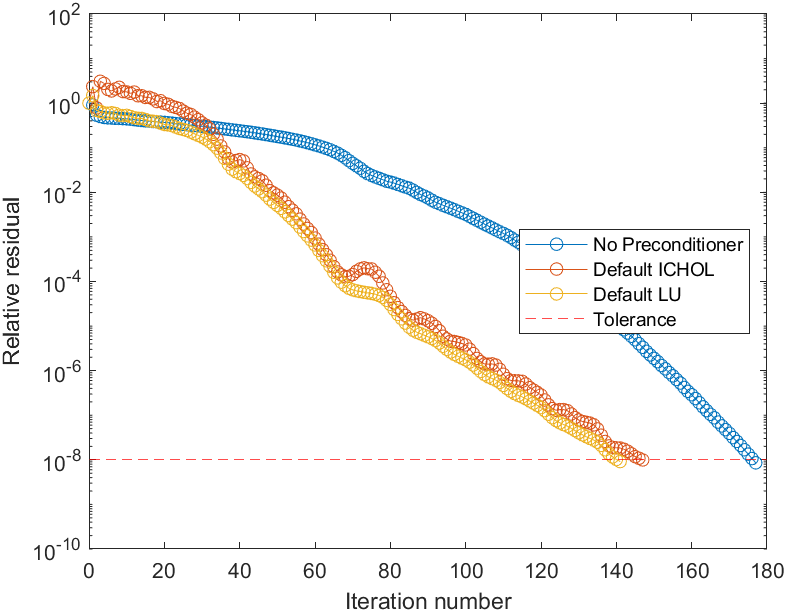
\includegraphics[scale=0.70]{img/dupcova/minres}}
    \caption{История невязок методом minres для матрицы Dubcova2}
    \label{fig:image_7}
\end{figure}

\begin{figure}[H]
    \renewcommand{\figurename}{Рисунок}
    \centering{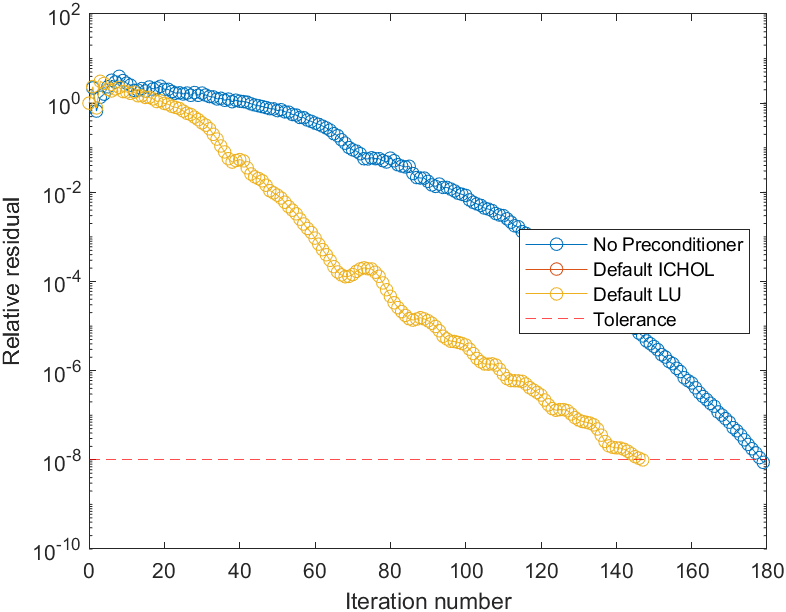
\includegraphics[scale=0.70]{img/dupcova/pcg}}
    \caption{История невязок методом pcg для матрицы Dubcova2}
    \label{fig:image_8}
\end{figure}

\begin{figure}[H]
    \renewcommand{\figurename}{Рисунок}
    \centering{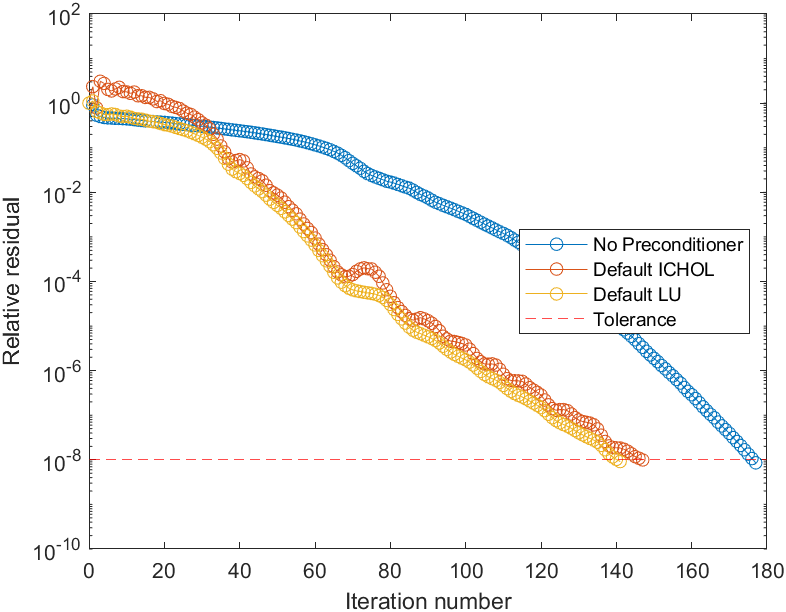
\includegraphics[scale=0.70]{img/dupcova/qmr}}
    \caption{История невязок методом qmr для матрицы Dubcova2}
    \label{fig:image_9}
\end{figure}

\begin{figure}[H]
    \renewcommand{\figurename}{Рисунок}
    \centering{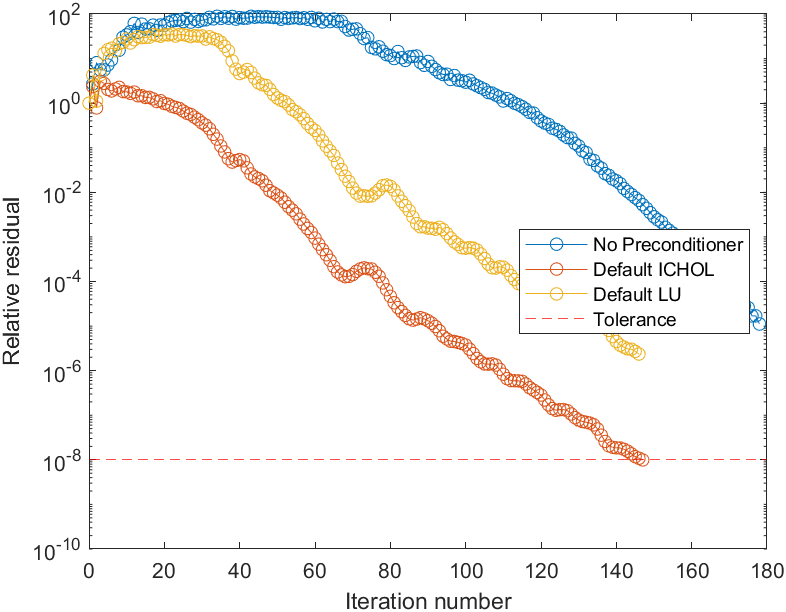
\includegraphics[scale=0.70]{img/dupcova/symmlq}}
    \caption{История невязок методом symmlq для матрицы Dubcova2}
    \label{fig:image_10}
\end{figure}

\begin{figure}[H]
    \renewcommand{\figurename}{Рисунок}
    \centering{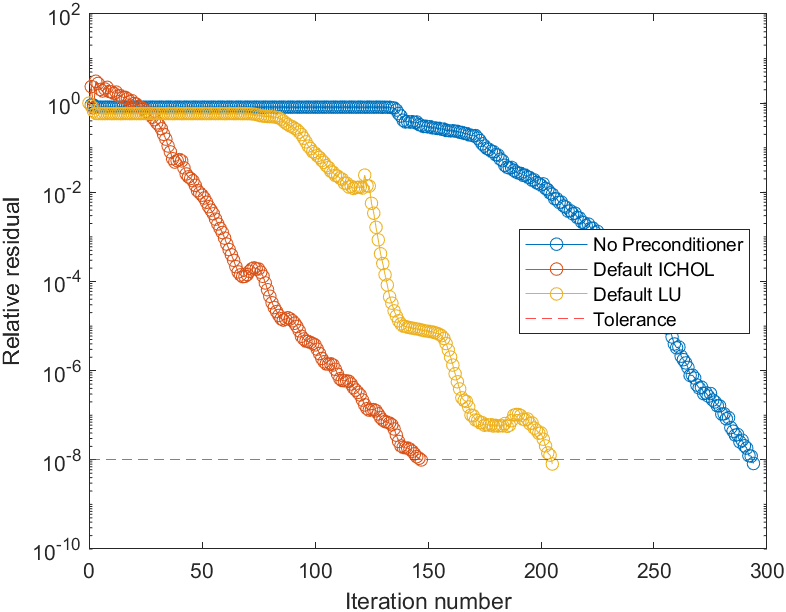
\includegraphics[scale=0.70]{img/dupcova/tfqmr}}
    \caption{История невязок методом tfqmr для матрицы Dubcova2}
    \label{fig:image_11}
\end{figure}
